% =========================================================================
% FIGURE & TEXT FILE FOR LATEX INPUT (\input{SoICT_2026/figure})
% Compatible with main.tex (uses subfigure package)
% =========================================================================

\usetikzlibrary{arrows.meta, calc}

% \setcounter{figure}{14} % Starts at Fig. 15

Figure~\ref{fig:seqrdf_initial} shows the initial network state with two active primary lightpaths: $\pi_1^W: C \to G$ and $\pi_2^W: A \to B \to C \to D \to E$ for requests $k_1$ and $k_2$. Links $C-D$ and $D-E$ support $W = 2$ wavelengths ($\pi_2^W$ uses $\lambda_0$), while all other links have $W = 1$. The sequential failure scenario considers directed link $\ell_1$ ($C \to G$) failing first, followed by $\ell_2$ ($A \to B$).


Figure~\ref{fig:seqrdf_fail_l1} and~\ref{fig:seqrdf_fail_l2} illustrates how a greedy first-stage restoration choice causes failure in stage 2. When $\ell_1$ fails (Fig.~\ref{fig:seqrdf_fail_l1}), $k_1$ takes the shortest backup $\pi_1^{R,(1)}: C \to B \to A \to G$, occupying link $A \to G$. When $\ell_2$ fails (Fig.~\ref{fig:seqrdf_fail_l2}), $k_2$ cannot restore because link $A \to B$ has failed and link $A \to G$ is blocked, leaving node $A$ with no available outgoing link.

\begin{figure}[t]
\centering
\vspace{-0.3em}
\subfigure[]{%
\label{fig:seqrdf_initial}%
\resizebox{0.48\textwidth}{!}{%
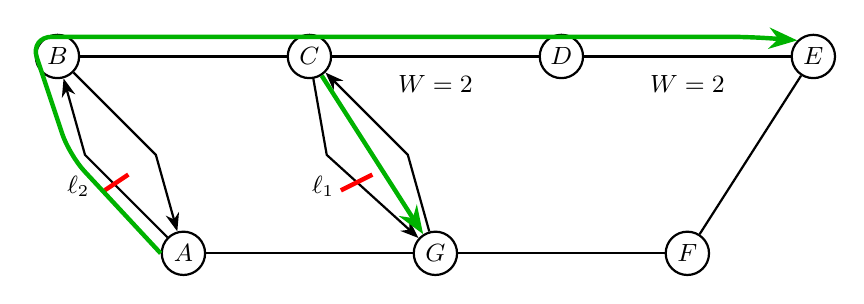
\begin{tikzpicture}[
    node/.style={circle, draw=black, thick, fill=white, minimum size=5.5mm, inner sep=1pt, font=\small\bfseries},
    dirlink/.style={->, >=Stealth, thick},
    link/.style={thick},
    failmark/.style={red, ultra thick},
    primary/.style={->, >=Stealth, ultra thick, color=green!70!black}
]
    % Hàng trên (B, C, D, E)
    \node[node] (B) at (0,   2.5) {$B$};
    \node[node] (C) at (3.2, 2.5) {$C$};
    \node[node] (D) at (6.4, 2.5) {$D$};
    \node[node] (E) at (9.6, 2.5) {$E$};

    % Hàng dưới (A, G, F)
    \node[node] (A) at (1.6, 0.0) {$A$};
    \node[node] (G) at (4.8, 0.0) {$G$};
    \node[node] (F) at (8.0, 0.0) {$F$};

    % Liên kết ngang hàng trên
    \draw[link] (B) -- (C);
    \draw[link] (C) -- (D) node[midway, below=3pt, font=\small\bfseries] {$W = 2$};
    \draw[link] (D) -- (E) node[midway, below=3pt, font=\small\bfseries] {$W = 2$};

    % Liên kết ngang & chéo hàng dưới
    \draw[link] (A) -- (G);
    \draw[link] (G) -- (F);
    \draw[link] (E) -- (F);

    % Cặp liên kết 2 hướng giữa B và A
    \draw[dirlink] (A) -- (0.35, 1.25) -- (B);
    \draw[dirlink] (B) -- (1.25, 1.25) -- (A);

    % Cặp liên kết 2 hướng giữa C và G
    \draw[dirlink] (C) -- (3.42, 1.25) -- (G);
    \draw[dirlink] (G) -- (4.45, 1.25) -- (C);

    % Đánh dấu lỗi \ell_2 và \ell_1
    \draw[failmark] (0.60, 0.80) -- (0.90, 1.0);;
    \node[left=2pt, font=\small\bfseries] at (0.60, 0.85) {$\ell_2$};

    \draw[failmark] (3.6, 0.80) -- (4.0, 1.0);
    \node[left=2pt, font=\small\bfseries] at (3.71, 0.85) {$\ell_1$};

    % Lightpath k1^w và k2^w
    \draw[primary] (C) -- (G);
    \draw[primary, rounded corners=8pt] (A.west) -- (0.15, 1.25) -- (-0.35, 2.75) -- (8.8, 2.75) -- (E.north west);

\end{tikzpicture}%
}
}
\subfigure[]{%
\label{fig:seqrdf_fail_l1}%
\resizebox{0.48\textwidth}{!}{%
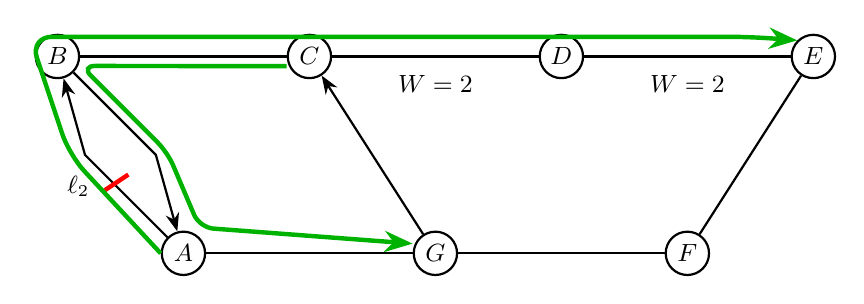
\begin{tikzpicture}[
    node/.style={circle, draw=black, thick, fill=white, minimum size=5.5mm, inner sep=1pt, font=\small\bfseries},
    dirlink/.style={->, >=Stealth, thick},
    link/.style={thick},
    failmark/.style={red, ultra thick},
    primary/.style={->, >=Stealth, ultra thick, color=green!70!black}
]
    \node[node] (B) at (0,   2.5) {$B$};
    \node[node] (C) at (3.2, 2.5) {$C$};
    \node[node] (D) at (6.4, 2.5) {$D$};
    \node[node] (E) at (9.6, 2.5) {$E$};

    \node[node] (A) at (1.6, 0.0) {$A$};
    \node[node] (G) at (4.8, 0.0) {$G$};
    \node[node] (F) at (8.0, 0.0) {$F$};

    \draw[link] (B) -- (C);
    \draw[link] (C) -- (D) node[midway, below=3pt, font=\small\bfseries] {$W = 2$};
    \draw[link] (D) -- (E) node[midway, below=3pt, font=\small\bfseries] {$W = 2$};

    \draw[link] (A) -- (G);
    \draw[link] (G) -- (F);
    \draw[link] (E) -- (F);

    \draw[dirlink] (A) -- (0.35, 1.25) -- (B);
    \draw[dirlink] (B) -- (1.25, 1.25) -- (A);

    \draw[dirlink] (G) -- (C);

    \draw[failmark] (0.60, 0.80) -- (0.90, 1.0);
    \node[left=2pt, font=\small\bfseries] at (0.60, 0.85) {$\ell_2$};

    \draw[primary, rounded corners=8pt] (A.west) -- (0.15, 1.25) -- (-0.35, 2.75) -- (8.8, 2.75) -- (E.north west);
    \draw[primary, rounded corners=5pt] ([yshift=-3.5pt]C.west) -- (0.3, 2.38) -- (1.40, 1.28) -- ([yshift=3.5pt]A.north east) -- ([yshift=3.5pt]G.west);
\end{tikzpicture}%
}%
}%
 \hfill
\subfigure[]{%
\label{fig:seqrdf_fail_l2}%
\resizebox{0.45\textwidth}{!}{%
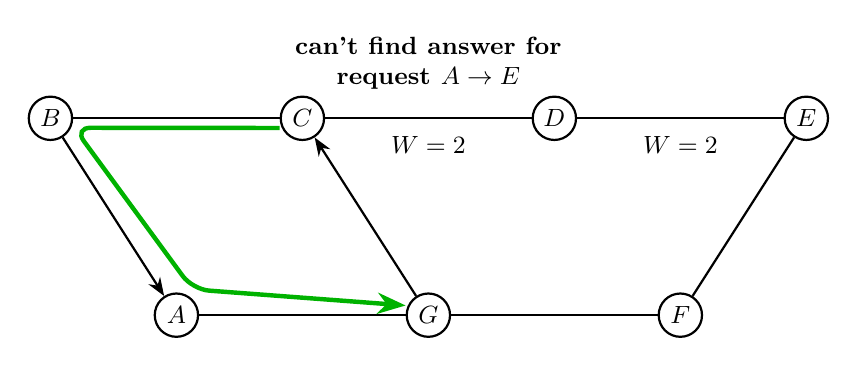
\begin{tikzpicture}[
    node/.style={circle, draw=black, thick, fill=white, minimum size=5.5mm, inner sep=1pt, font=\small\bfseries},
    dirlink/.style={->, >=Stealth, thick},
    link/.style={thick},
    failmark/.style={red, ultra thick},
    primary/.style={->, >=Stealth, ultra thick, color=green!70!black}
]
    \node[node] (B) at (0,   2.5) {$B$};
    \node[node] (C) at (3.2, 2.5) {$C$};
    \node[node] (D) at (6.4, 2.5) {$D$};
    \node[node] (E) at (9.6, 2.5) {$E$};

    \node[node] (A) at (1.6, 0.0) {$A$};
    \node[node] (G) at (4.8, 0.0) {$G$};
    \node[node] (F) at (8.0, 0.0) {$F$};

    \node[font=\small\bfseries, align=center] at (4.8, 3.2) {can't find answer for\\request $A \to E$};

    \draw[link] (B) -- (C);
    \draw[link] (C) -- (D) node[midway, below=3pt, font=\small\bfseries] {$W = 2$};
    \draw[link] (D) -- (E) node[midway, below=3pt, font=\small\bfseries] {$W = 2$};

    \draw[link] (A) -- (G);
    \draw[link] (G) -- (F);
    \draw[link] (E) -- (F);

    \draw[dirlink] (B) -- (A);
    \draw[dirlink] (G) -- (C);

    \draw[primary, rounded corners=6pt] ([yshift=-3.5pt]C.west) -- (0.3, 2.38) -- ([yshift=3.5pt]A.north east) -- ([yshift=3.5pt]G.west);
\end{tikzpicture}%
}%
}%
% \hfill
\quad
\subfigure[]{%
\label{fig:seqrdf_good}%
\resizebox{0.45\textwidth}{!}{%
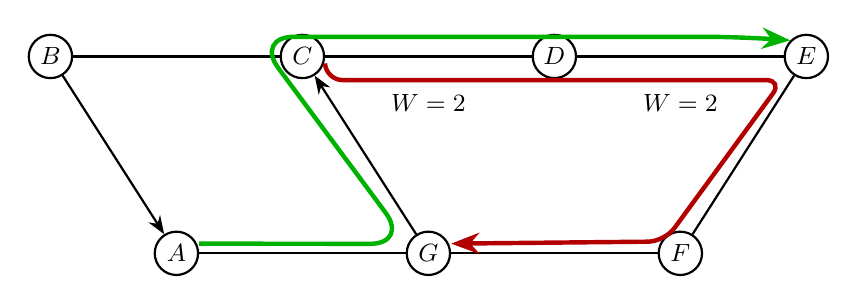
\begin{tikzpicture}[
    node/.style={circle, draw=black, thick, fill=white, minimum size=5.5mm, inner sep=1pt, font=\small\bfseries},
    dirlink/.style={->, >=Stealth, thick},
    link/.style={thick},
    failmark/.style={red, ultra thick},
    primary/.style={->, >=Stealth, ultra thick, color=green!70!black},
    primary_red/.style={->, >=Stealth, ultra thick, color=red!70!black}
]
    \node[node] (B) at (0,   2.5) {$B$};
    \node[node] (C) at (3.2, 2.5) {$C$};
    \node[node] (D) at (6.4, 2.5) {$D$};
    \node[node] (E) at (9.6, 2.5) {$E$};

    \node[node] (A) at (1.6, 0.0) {$A$};
    \node[node] (G) at (4.8, 0.0) {$G$};
    \node[node] (F) at (8.0, 0.0) {$F$};

    \draw[link] (B) -- (C);
    \draw[link] (C) -- (D) node[midway, below=10pt, font=\small\bfseries] {$W = 2$};
    \draw[link] (D) -- (E) node[midway, below=10pt, font=\small\bfseries] {$W = 2$};

    \draw[link] (A) -- (G);
    \draw[link] (G) -- (F);
    \draw[link] (E) -- (F);

    \draw[dirlink] (B) -- (A);
    \draw[dirlink] (G) -- (C);

    \draw[primary, rounded corners=14pt] ([yshift=3.5pt]A.east) -- (4.55, 0.12) -- (2.60, 2.75) -- (8.8, 2.75) -- (E.north west);
    \draw[primary_red, rounded corners=6pt] ([yshift=-3.5pt]C.east) -- (3.5, 2.20) -- (9.30, 2.20) -- (7.80, 0.15) -- ([yshift=3.5pt]G.east);
\end{tikzpicture}%
}%
}%
\vspace{-0.3em}
\caption{Suboptimal first-stage backup for $k_1$ leading to restoration failure of $k_2$.}
\label{fig:seqrdf_example}
\end{figure}

Figure~\ref{fig:seqrdf_good} shows that choosing a longer first-stage backup enables full recovery. When $\ell_1$ fails, $k_1$ takes $\pi_1^{R,(1)}: C \to D \to E \to F \to G$ on $\lambda_1$, keeping link $A \to G$ free. When $\ell_2$ fails, $\pi_2^W$ is disrupted (releasing $\lambda_0$ on $C-D, D-E$) and successfully restores via $\pi_2^{R,F}: A \to G \to C \to D \to E$ on $\lambda_0$. Both requests are thus fully recovered.
This example is to show that taking the shortest path as a restoration path is not always a good choice.

% \begin{figure}[htbp]
% \centering
% \vspace{-0.3em}
% \subfigure[]{%
% \label{fig:seq2_a}%
% \resizebox{0.48\textwidth}{!}{%
% \begin{tikzpicture}[
%     node/.style={circle, draw=black, thick, fill=white, minimum size=5.5mm, inner sep=1pt, font=\small\bfseries},
%     dirlink/.style={->, >=Stealth, thick},
%     link/.style={thick},
%     failmark/.style={red, ultra thick},
%     primary/.style={->, >=Stealth, ultra thick, color=green!70!black},
%     primary_red/.style={->, >=Stealth, ultra thick, color=red!70!black}
% ]
%     \node[node] (B) at (0,   2.5) {$B$};
%     \node[node] (C) at (3.2, 2.5) {$C$};
%     \node[node] (D) at (6.4, 2.5) {$D$};
%     \node[node] (E) at (9.6, 2.5) {$E$};

%     \node[node] (A) at (1.6, 0.0) {$A$};
%     \node[node] (G) at (4.8, 0.0) {$G$};
%     \node[node] (F) at (8.0, 0.0) {$F$};

%     \draw[link] (B) -- (C);
%     \draw[link] (C) -- (D) node[midway, below=10pt, font=\small\bfseries] {$W = 2$};
%     \draw[link] (D) -- (E) node[midway, below=10pt, font=\small\bfseries] {$W = 2$};

%     \draw[link] (A) -- (G);
%     \draw[link] (G) -- (F);
%     \draw[link] (E) -- (F);

%     \draw[dirlink] (A) -- (0.35, 1.25) -- (B);
%     \draw[dirlink] (B) -- (1.25, 1.25) -- (A);

%     \draw[dirlink] (G) -- (C);

%     \draw[failmark] (0.70, 0.80) -- (0.80, 0.90);
%     \node[left=2pt, font=\small\bfseries] at (0.60, 0.85) {$\ell_2$};

%     \draw[primary, rounded corners=8pt] (A.west) -- (0.15, 1.25) -- (-0.35, 2.78) -- (8.8, 2.78) -- (E.north west);
%     \draw[primary_red, rounded corners=6pt] ([yshift=-3.5pt]C.east) -- (3.5, 2.20) -- (9.30, 2.20) -- (7.80, 0.15) -- ([yshift=3.5pt]G.east);
% \end{tikzpicture}%
% }%
% }%
% \hfill
% \subfigure[]{%
% \label{fig:seq2_b}%
% \resizebox{0.48\textwidth}{!}{%
% \begin{tikzpicture}[
%     node/.style={circle, draw=black, thick, fill=white, minimum size=5.5mm, inner sep=1pt, font=\small\bfseries},
%     dirlink/.style={->, >=Stealth, thick},
%     link/.style={thick},
%     failmark/.style={red, ultra thick},
%     primary/.style={->, >=Stealth, ultra thick, color=green!70!black},
%     primary_red/.style={->, >=Stealth, ultra thick, color=red!70!black}
% ]
%     \node[node] (B) at (0,   2.5) {$B$};
%     \node[node] (C) at (3.2, 2.5) {$C$};
%     \node[node] (D) at (6.4, 2.5) {$D$};
%     \node[node] (E) at (9.6, 2.5) {$E$};

%     \node[node] (A) at (1.6, 0.0) {$A$};
%     \node[node] (G) at (4.8, 0.0) {$G$};
%     \node[node] (F) at (8.0, 0.0) {$F$};

%     \draw[link] (B) -- (C);
%     \draw[link] (C) -- (D) node[midway, below=10pt, font=\small\bfseries] {$W = 2$};
%     \draw[link] (D) -- (E) node[midway, below=10pt, font=\small\bfseries] {$W = 2$};

%     \draw[link] (A) -- (G);
%     \draw[link] (G) -- (F);
%     \draw[link] (E) -- (F);

%     \draw[dirlink] (B) -- (A);
%     \draw[dirlink] (G) -- (C);

%     \draw[primary, rounded corners=14pt] ([yshift=3.5pt]A.east) -- (4.55, 0.12) -- (2.60, 2.75) -- (8.8, 2.75) -- (E.north west);
%     \draw[primary_red, rounded corners=6pt] ([yshift=-3.5pt]C.east) -- (3.5, 2.20) -- (9.30, 2.20) -- (7.80, 0.15) -- ([yshift=3.5pt]G.east);
% \end{tikzpicture}%
% }%
% }%
% \vspace{-0.3em}
% \caption{Optimal first-stage backup for $k_1$ enabling successful recovery of both requests.}
% \label{fig:seq2_full}
% \end{figure}

